% !TeX encoding = UTF-8
% !TeX root = summary.tex
% !TeX spellcheck = en_US

%---------------------------------------------------------------------------------------------------
% Preamble
%---------------------------------------------------------------------------------------------------

\documentclass[9pt,a4paper]{extarticle}

\usepackage[english]{babel}
\usepackage{graphicx}
\usepackage[T1]{fontenc}
\usepackage{times}
\usepackage[utf8]{inputenc}
\usepackage{url}
\usepackage{multicol}
\usepackage{float}
\usepackage[tableposition=top]{caption}
\usepackage[a4paper,margin=30mm,noheadfoot]{geometry}
\usepackage[noabbrev,nameinlink]{cleveref}

\columnsep 12mm
\pagestyle{empty}
\captionsetup{figurename=Fig.,tablename=Tab.,labelsep=endash,font=bf,skip=.5\baselineskip,justification=centering}

\makeatletter
\renewcommand*{\@seccntformat}[1]{%
  \csname the#1\endcsname.\quad
}
\makeatother

\clubpenalty=300
\widowpenalty=300

\graphicspath{{figures/}}
\setlength{\belowcaptionskip}{-5pt}


%---------------------------------------------------------------------------------------------------
% Header
%---------------------------------------------------------------------------------------------------


\begin{document}

\begin{center}
  \huge{\textbf{\textsc{Robot Self-Localization in Dynamic Environments}}}\\[4mm]
  \Large{\emph{Carlos Miguel Correia da Costa}}\\[2mm]
  \normalsize{Dissertation conducted under the supervision of \emph{Doctor Armando Jorge Miranda de Sousa}\\and co-supervision of \emph{Doctor Germano Manuel Correia dos Santos Veiga}}\\
  \normalsize{at \emph{Centre for Robotics and Intelligent Systems of INESC-TEC}}
\end{center}

\thispagestyle{empty}
\vspace*{-4mm}\noindent\rule{\textwidth}{0.4pt}\vspace*{4mm}



%---------------------------------------------------------------------------------------------------
% Summary
%---------------------------------------------------------------------------------------------------


\begin{multicols}{2}

\section{Context}

Humanity has sought a reliable method of navigation ever since it started to explore the world. It began with simple landmark reference points for local travels, then perfected celestial navigation for global journeys, and when it finally conquered space, it deployed an accurate global localization system. Autonomous robots face the same problem, because in order to be able to navigate with precision, they first need to know their location. Over the years, several localization methods have been proposed and refined, according to the navigation environment and the accuracy requirements. Some are meant for high precision local navigation, while others provide an approximate global position.

A robot capable of operating safely and accurately in a dynamic environment can have innumerous applications, ranging from simple delivery tasks to advanced assembly. Besides improving productivity by performing repetitive tasks with precision and speed, robots can also act as coworkers, helping humans perform their jobs more efficiently and thus, reducing the overall production costs.


\section{Project}

CARLoS\footnote{\url{http://carlosproject.eu/}} is a European research project that aims to develop an autonomous robot capable of performing repetitive tasks alongside human co-workers in dynamic environments. The robot will operate in shipyards and is intended to perform fit-out operations, such as stud welding and projection mapping of CAD drawings. Stud welding is a repetitive task that provides structural support for other components, such as heat insulation layers or electrical systems. Projection mapping of CAD drawings or other important information will help human co-workers assemble components faster, because it will mark the exact position in which they must be installed.


\section{Motivation and objectives}

With the increase of competitiveness in the current globalized trading markets, companies are trying to reduce production costs and improve the productivity of their assets. Robots can help achieve these goals by performing the simple and repetitive jobs while giving humans more free time to perform the complex and creative tasks.

Mobile platforms equipped with robotic arms provide a flexible way to automate a wide range of tasks that must be performed over large areas. However, before performing the intended operations they first need to know where they are and how they can reach the desired location. Moreover, given their limited computational resources and energy storages, they require efficient, reliable and accurate control systems capable to operate in real time.



\section{Contributions}

During this dissertation it was developed an efficient, modular and extensible 3/6 DoF localization system\footnote{\url{https://github.com/carlosmccosta/dynamic_robot_localization}} for mobile robot platforms capable of operating accurately and reliably in dynamic environments. It is a multi-level registration pipeline that uses geometric features to estimate the initial position of a robot platform and point cloud registration algorithms to track its pose. The tracking subsystem can have two different configurations. One tuned for maximum efficiency used for the normal operation of the mobile platform and another for unlikely situations that may require more robust registration algorithms / configurations. It also supports incremental map update and can adjust its operation rate based on the estimated robot velocity. For critical operations, it provides a detailed analysis of the tracking quality and when initial pose estimation is required it gives the distribution of the acceptable poses, which can be very valuable information if there are several areas in the known map with very similar geometry.


\section{Testing platforms}

The localization system was tested on laser sensor data retrieved from three different mobile robot platforms (shown from \crefrange{fig:jarvis}{fig:guardian-gazebo}) and also from a Kinect. The tests were performed on the same computer in order to allow a direct comparison of computation time. This computer was a Clevo P370EM3 laptop (with a Intel Core i7 3630QM CPU at 2.4GHz, 16 GB of RAM DDR3, NVidia GTX680M graphics card and a Samsung 840 Pro SSD) and it was running Ubuntu 12.04 along with ROS Hydro, PCL 1.7 and Gazebo 1.9.

The sensor data was recorded into rosbags, and is publicly available at\footnote{\url{https://github.com/carlosmccosta/dynamic_robot_localization_tests}} along with all the detailed results and experiments videos, in order to allow future comparisons with other localization systems.

\begin{figure}[H]
	\centering
	\begin{minipage}[b]{0.23\textwidth}
		\centering
		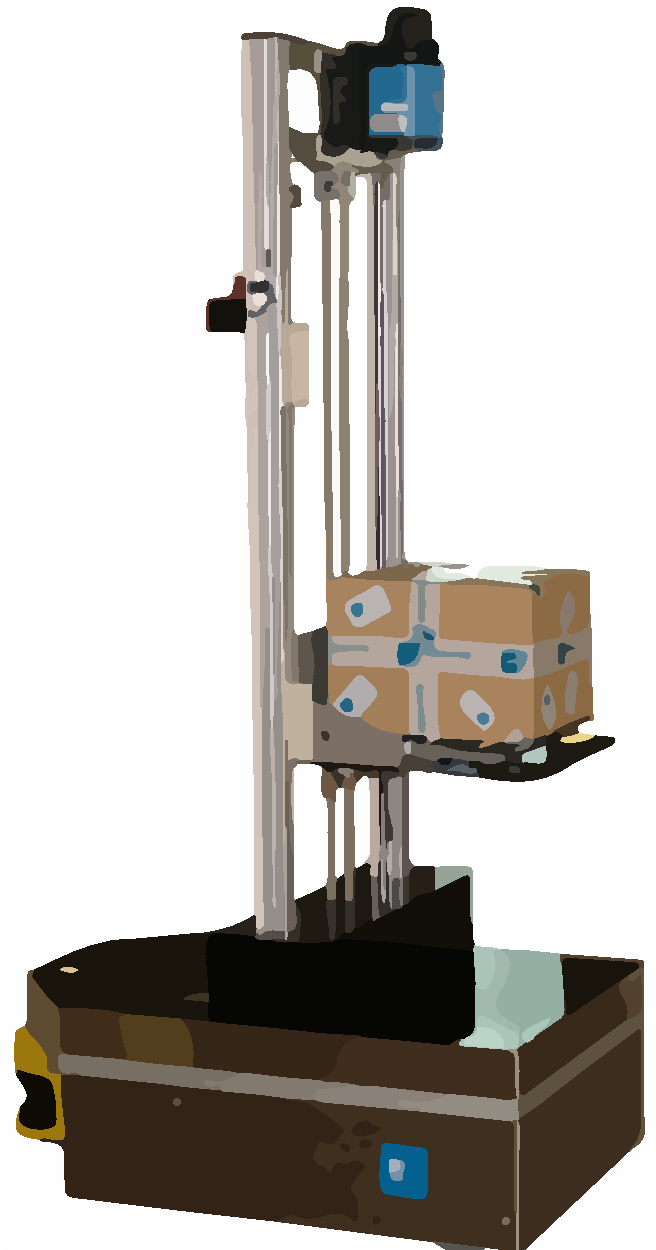
\includegraphics[width=0.35\textwidth]{jarvis}
		\caption{\small Jarvis robot}
		\label{fig:jarvis}
	\end{minipage}\hfill
	\begin{minipage}[b]{0.23\textwidth}
		\centering
		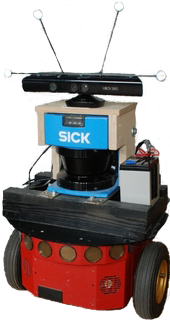
\includegraphics[width=0.27\textwidth]{pioneer-3dx}
		\caption{\small Pioneer robot \cite{Sturm2012}}
		\label{fig:pioneer}
	\end{minipage}
\end{figure}

\begin{figure}[H]
	\centering
	\begin{minipage}[b]{0.2\textwidth}
		\centering
		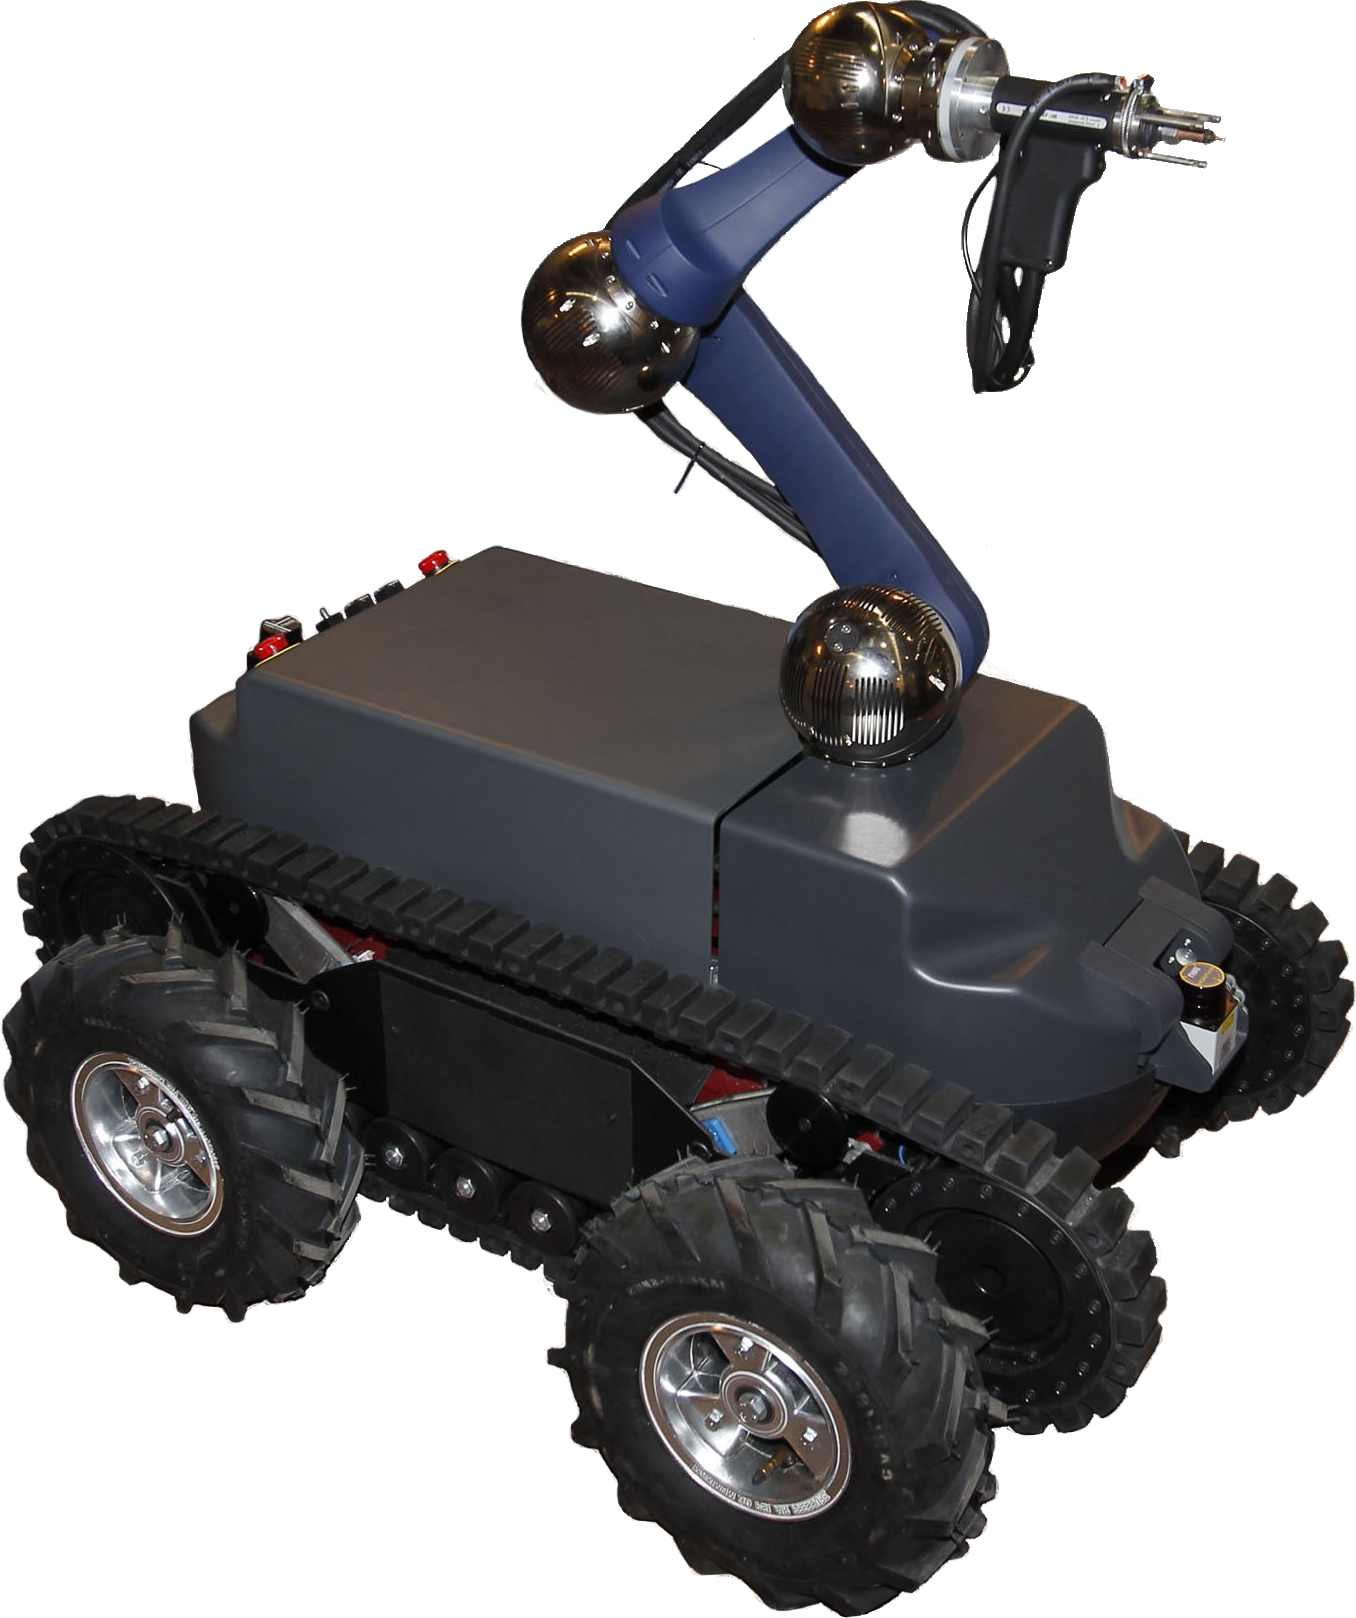
\includegraphics[width=0.6\textwidth]{guardian}
		\caption{\small Guardian robot}
		\label{fig:guardian}
	\end{minipage}\hfill
	\begin{minipage}[b]{0.25\textwidth}
		\centering
		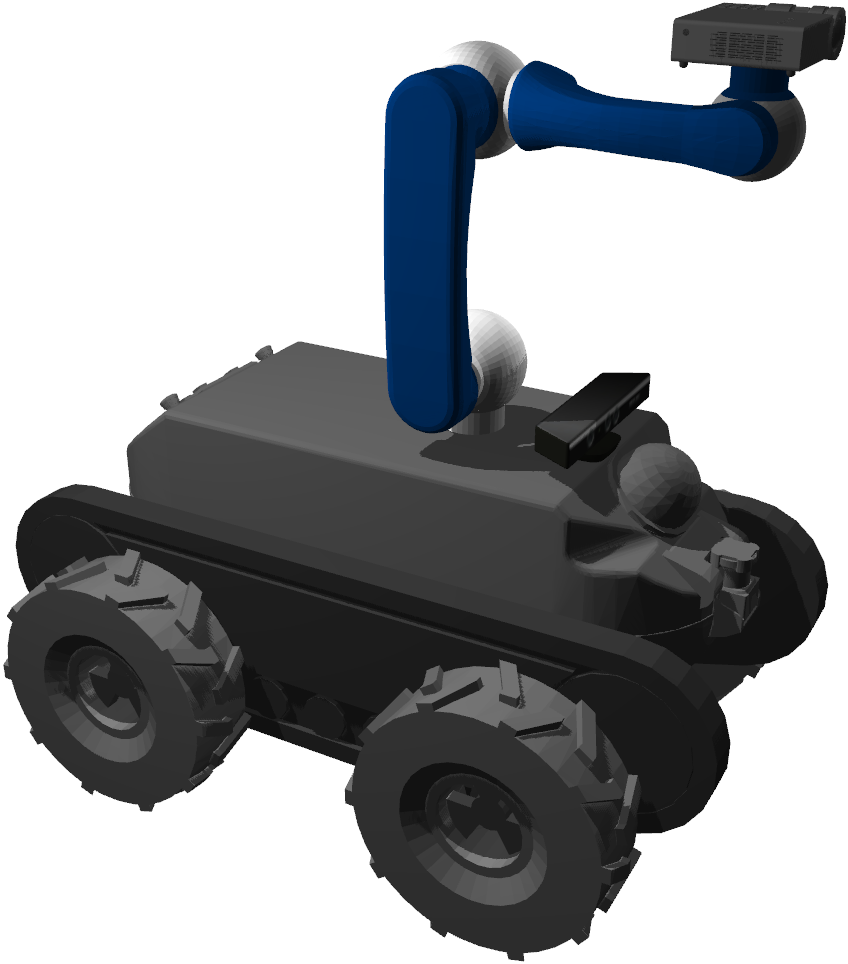
\includegraphics[width=0.45\textwidth]{guardian-gazebo}
		\caption{\small Guardian simulation}
		\label{fig:guardian-gazebo}
	\end{minipage}
\end{figure}


\section{Testing environments}

The localization system was tested in different environments (shown from \crefrange{fig:jarvis-environment}{fig:kinect-environment}) and used the Jarvis platform in a large room with a RoboCup field, the Pioneer 3-DX in a large industrial hall, the Guardian platform in a simulated indoor environment and a Kinect in a flying arena.


\begin{figure}[H]
	\centering
	\begin{minipage}[b]{0.23\textwidth}
		\centering
		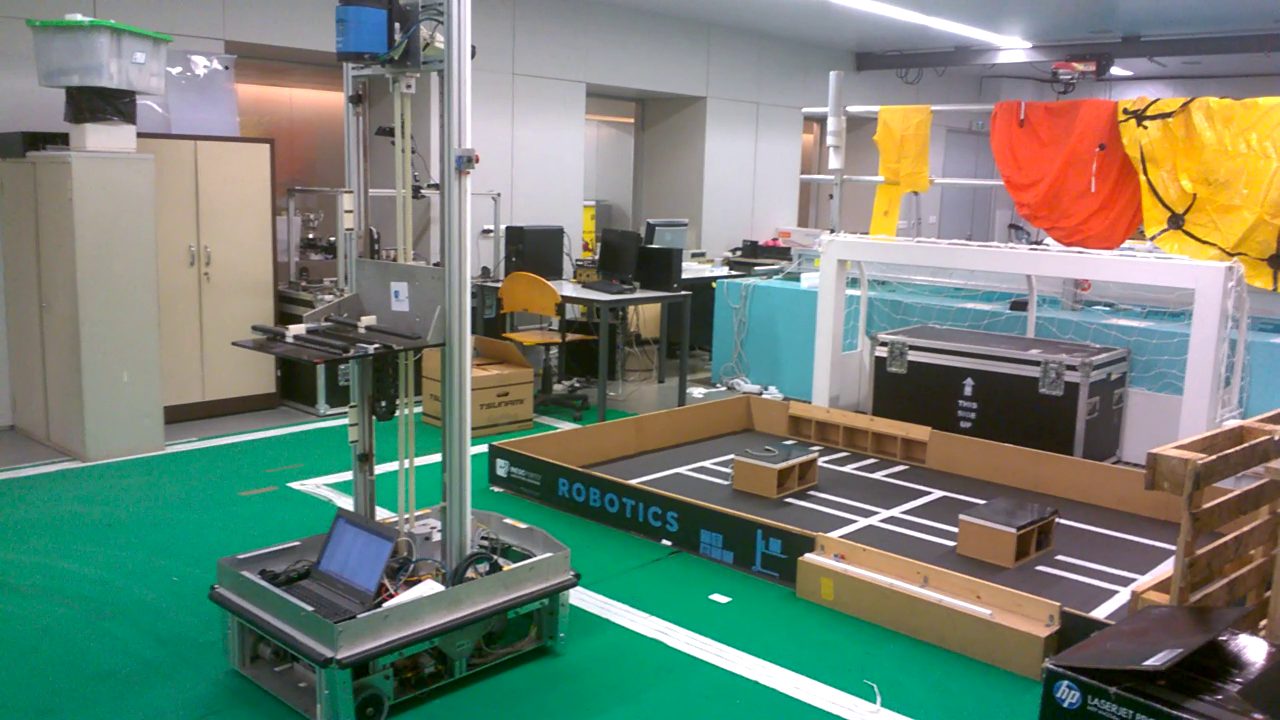
\includegraphics[width=\textwidth]{jarvis-environment-front-right}
		\caption{\small RoboCup field}
		\label{fig:jarvis-environment}
	\end{minipage}\hfill
	\begin{minipage}[b]{0.23\textwidth}
		\centering
		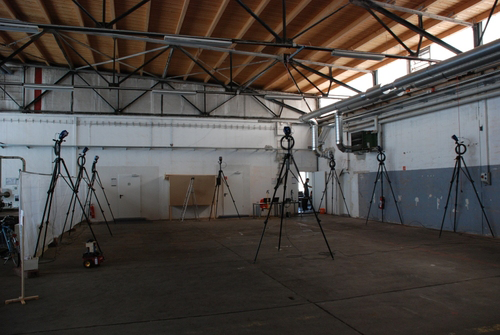
\includegraphics[width=0.85\textwidth]{industrial-hall}
		\caption{\small Industrial hall \cite{Sturm2012}}
		\label{fig:pioneer-environment}
	\end{minipage}
\end{figure}


\begin{figure}[H]
	\centering
	\begin{minipage}[b]{0.23\textwidth}
		\centering
		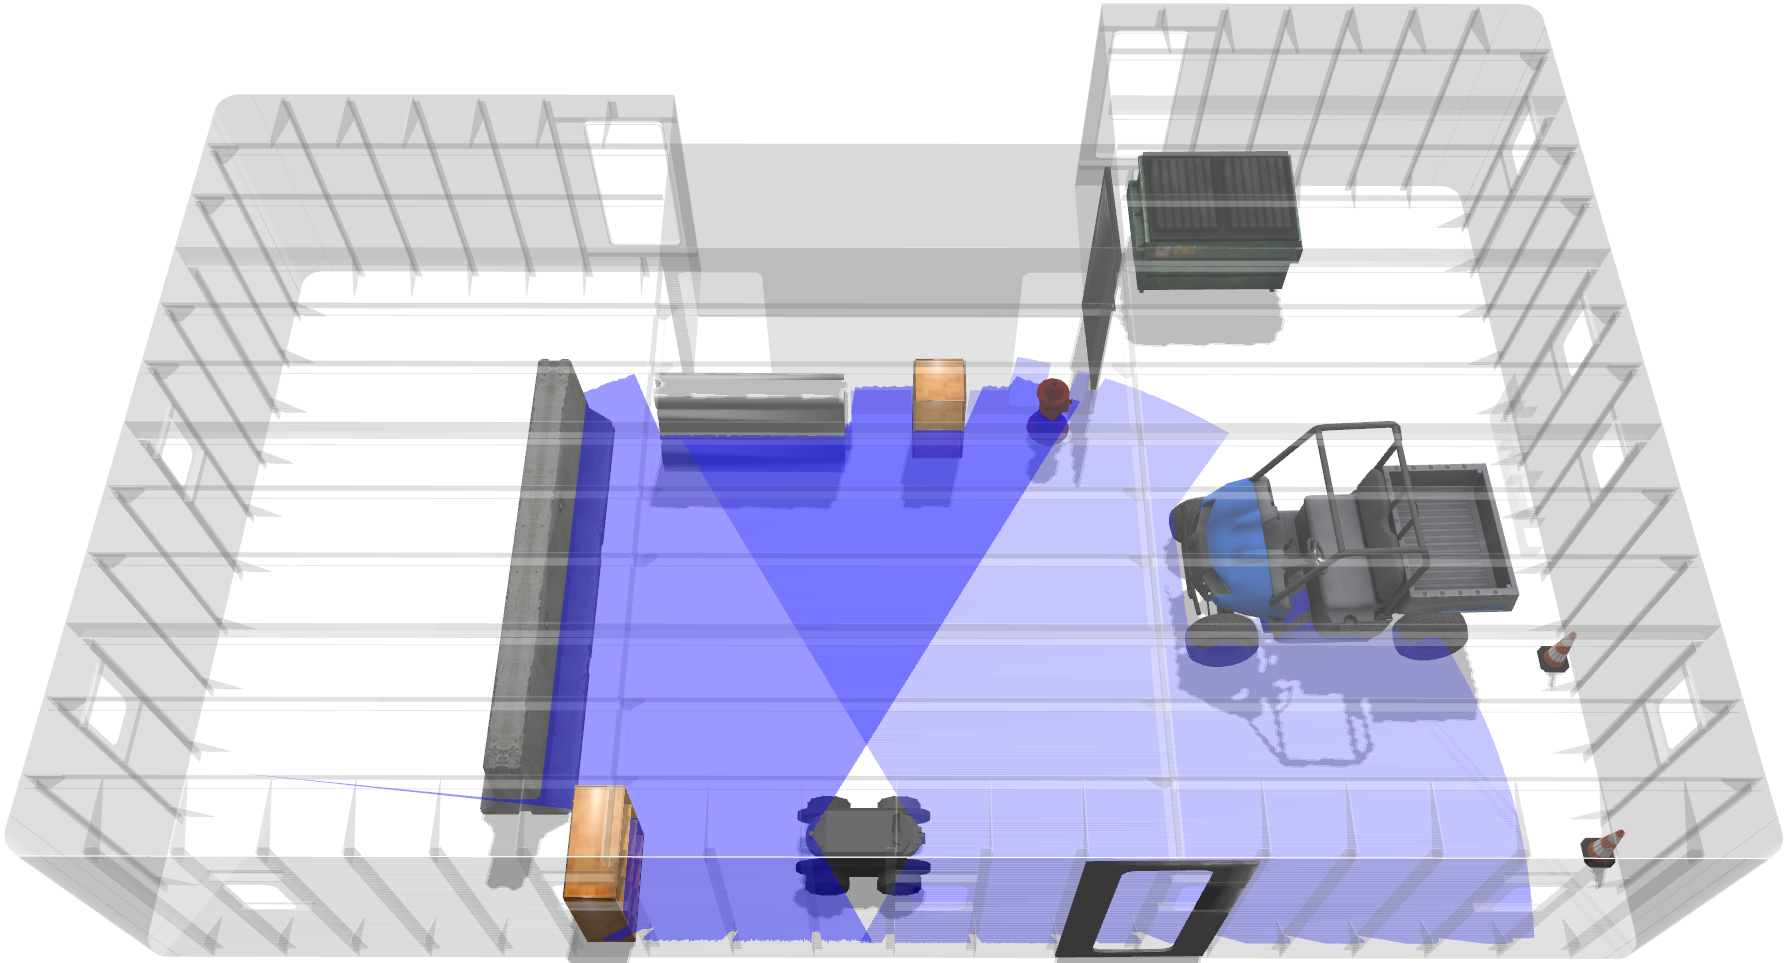
\includegraphics[width=\textwidth]{guardian-environment-cluttered-dynamic}
		\caption{\small Indoor environment}
		\label{fig:guardian-environment}
	\end{minipage}\hfill
	\begin{minipage}[b]{0.23\textwidth}
		\centering
		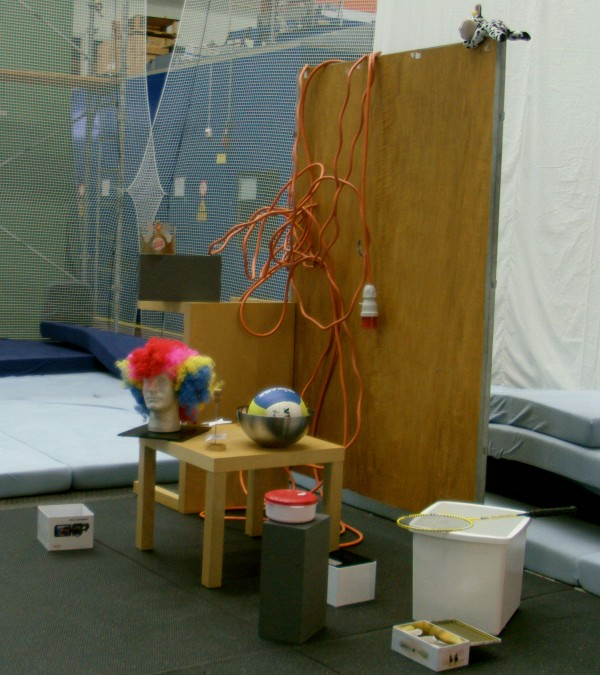
\includegraphics[width=0.6\textwidth]{kinect-flying-arena}
		\caption{\small Flying arena \cite{Pomerleau2011}}
		\label{fig:kinect-environment}
	\end{minipage}
\end{figure}



\section{Main results}

The proposed localization system is able to maintain pose tracking with less than 1-2 centimeters of translation error and less than a 1-3 degrees of rotation error (in 3 and 6 DoF respectively) even when the robot / sensors are moving at high velocities in cluttered and dynamic environments. Moreover, when tracking is lost or no initial pose is given, the system is able to find a valid global pose estimate by switching to more robust registration algorithms that use feature matching. This approach achieved fast pose tracking and reliable initial pose estimation while also providing the set of the accepted initial poses before registration refinement, which can be very valuable information for a navigation supervisor when the robot is in an ambiguous region that can be registered in similar zones of the known map. The system also allows dynamic reconfiguration of the number of laser scans to assemble in order to mitigate laser measurement errors and can adapt its rate of operation according to the robot estimated velocity.


\section{Conclusions}

The sub-centimeter accuracy achieved by the proposed localization system along with the dynamic map update capability and the need of no artificial landmarks / ambient modifications will allow the fast deployment of mobile robots capable to operate safely and accurately in cluttered environments.


\section{Future work}

The current implementation of the self-localization system can be further improved with GPU support \cite{Tamaki2010} in order to achieve higher update rates in 6 DoF and also with loop closing algorithms \cite{Grisetti2012} in order to become a complete SLAM system and allow the creation of accurate maps of very large environments. Moreover, it could be extended to support image based localization \cite{Labb2014} and semantic perception / mapping of the environment \cite{Santos2013}.


\bibliographystyle{unsrt}
\bibliography{references}

\end{multicols}

\end{document}
